\section{Laboratory work implementation}

\subsection{Tasks and Points}

\begin{enumerate}
\item Realizarea unui site
\item Site-ul trebuie să păstreze toată informația într-o baza de date
\item Site-ul trebuie să conțină AJAX Requests.
\item Implementarea XHR sau JSON responses. Careva din informație trebuie să fie dinamic încărcată pe pagină.
\end{enumerate}

\subsection{Analiza lucrarii de laborator}

\begin{enumerate}
\item Primul pas a fost inițializarea unui nou repozitoriu pe GitHub și clonarea acestuia pe calculatorul personal: \url{https://github.com/emirovschi/MIDPS\-3}.
\item Proiectul a fost creat utilizând IntelliJ\cite{IntelliJ} și folosind Maven\cite{Maven} ca build manager. Acesta oferă posibilitatea de a adăuga automat toate dependențele inclusiv cele tranzitive.
\item Backend-ul este bazat pe Spring framework. Acesta oferă un sistem de dependency injection\cite{IoC} care oferă posibilitatea de a crea ușor componente și de a suplini dependențele acestora. O altă parte necesară din framework este integrarea pattern-ului MVC\cite{MVC} care permite  crearea unui REST API.

\begin{minipage}{\linewidth}
	\centering
	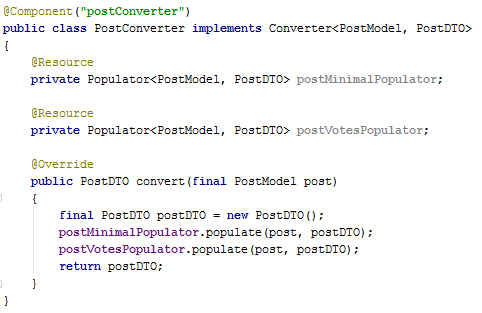
\includegraphics{inject}
	\captionof{figure}{Crearea componentelor și injectarea dependențelor folosind Spring framework}
\end{minipage}
\break

\begin{minipage}{\linewidth}
	\centering
	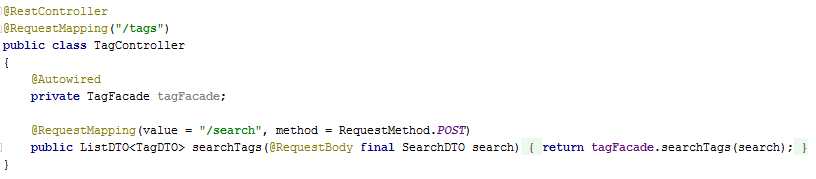
\includegraphics{rest}
	\captionof{figure}{Definirea unui REST endpoint}
\end{minipage}
\break

\item Spring oferă posibilitatea de a defini entități folosind JPA framework\cite{JPA} și repozitorii care vor gestiona aceste entități. Astfel acest framework permite implementarea proiectului fără a depinde de o anumită bază de date. În acest caz am utilizat local pentru dezvoltare și testare o baza de date de tip H2 însă pe server se folosește PostgresSQL fără a efectua careva schimbări majore cu excepția configurărilor.

\begin{minipage}{\linewidth}
	\centering
	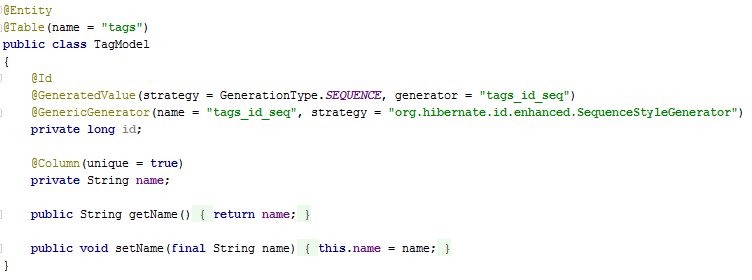
\includegraphics{entity}
	\captionof{figure}{Definirea unei entități}
\end{minipage}
\break

\begin{minipage}{\linewidth}
	\centering
	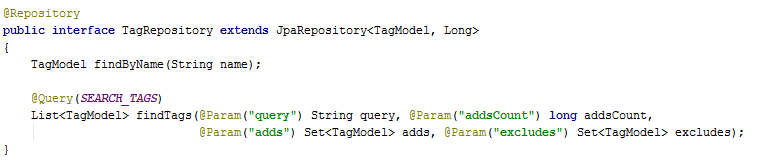
\includegraphics{repository}
	\captionof{figure}{Definirea unui repozitoriu}
\end{minipage}
\break

\item O altă funcționalitate importantă oferită de acest framework este Spring Boot\cite{boot} care înclude în sine HTTP server și elimină dependeța de careva aplicație gen Tomcat.
\item Partea front-end a fost implementată utilizând framework-ul AngularJS\cite{AngularJS}. Aceta oferă posibilitatea de a crea un single page application utilizând MVW pattern.

\begin{minipage}{\linewidth}
	\centering
	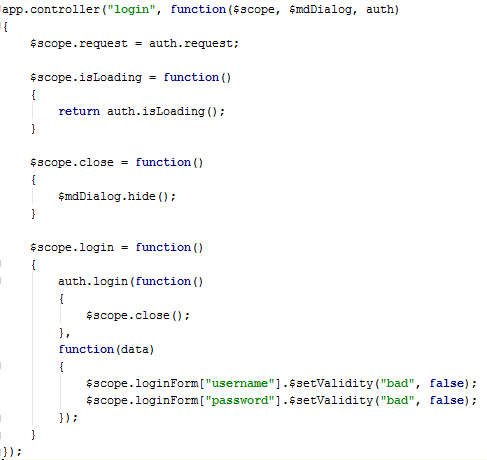
\includegraphics{controller}
	\captionof{figure}{Exemplu de controller}
\end{minipage}
\break

\begin{minipage}{\linewidth}
	\centering
	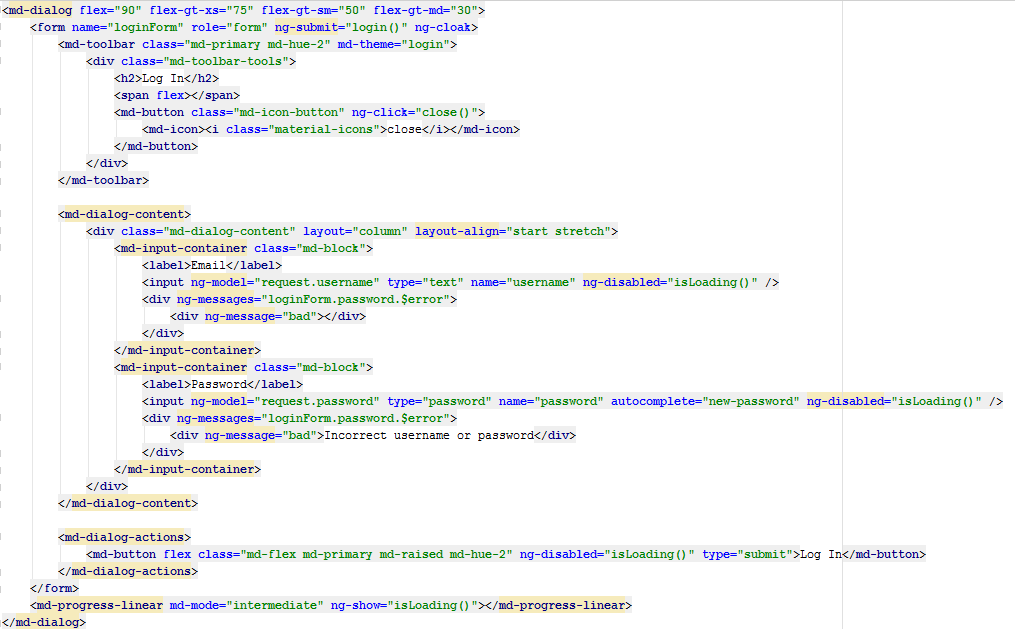
\includegraphics[width=17cm]{template}
	\captionof{figure}{Exemplu de template}
\end{minipage}
\break

\item Pentru ușura definirea elementelor a fost inclusă extensia Angular Material\cite{AngularMaterial} care oferă un set de componente web, instrucțiuni de definire a structurii pagini și a stilurilor acesteia inclusiv pentru diferite dispozitive.

\begin{minipage}{\linewidth}
	\centering
	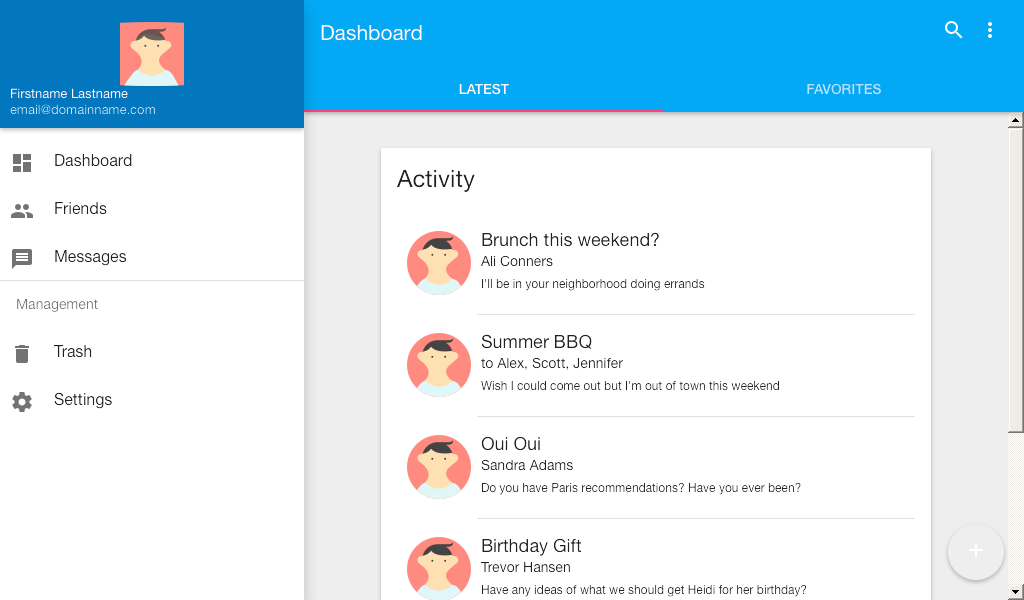
\includegraphics[width=17cm]{material}
	\captionof{figure}{Exemplu de pagină creată folosind Angular Material}
\end{minipage}
\break

\end{enumerate}

\break
\subsection{Imagini}

\begin{figure}[ht]
	\centering
	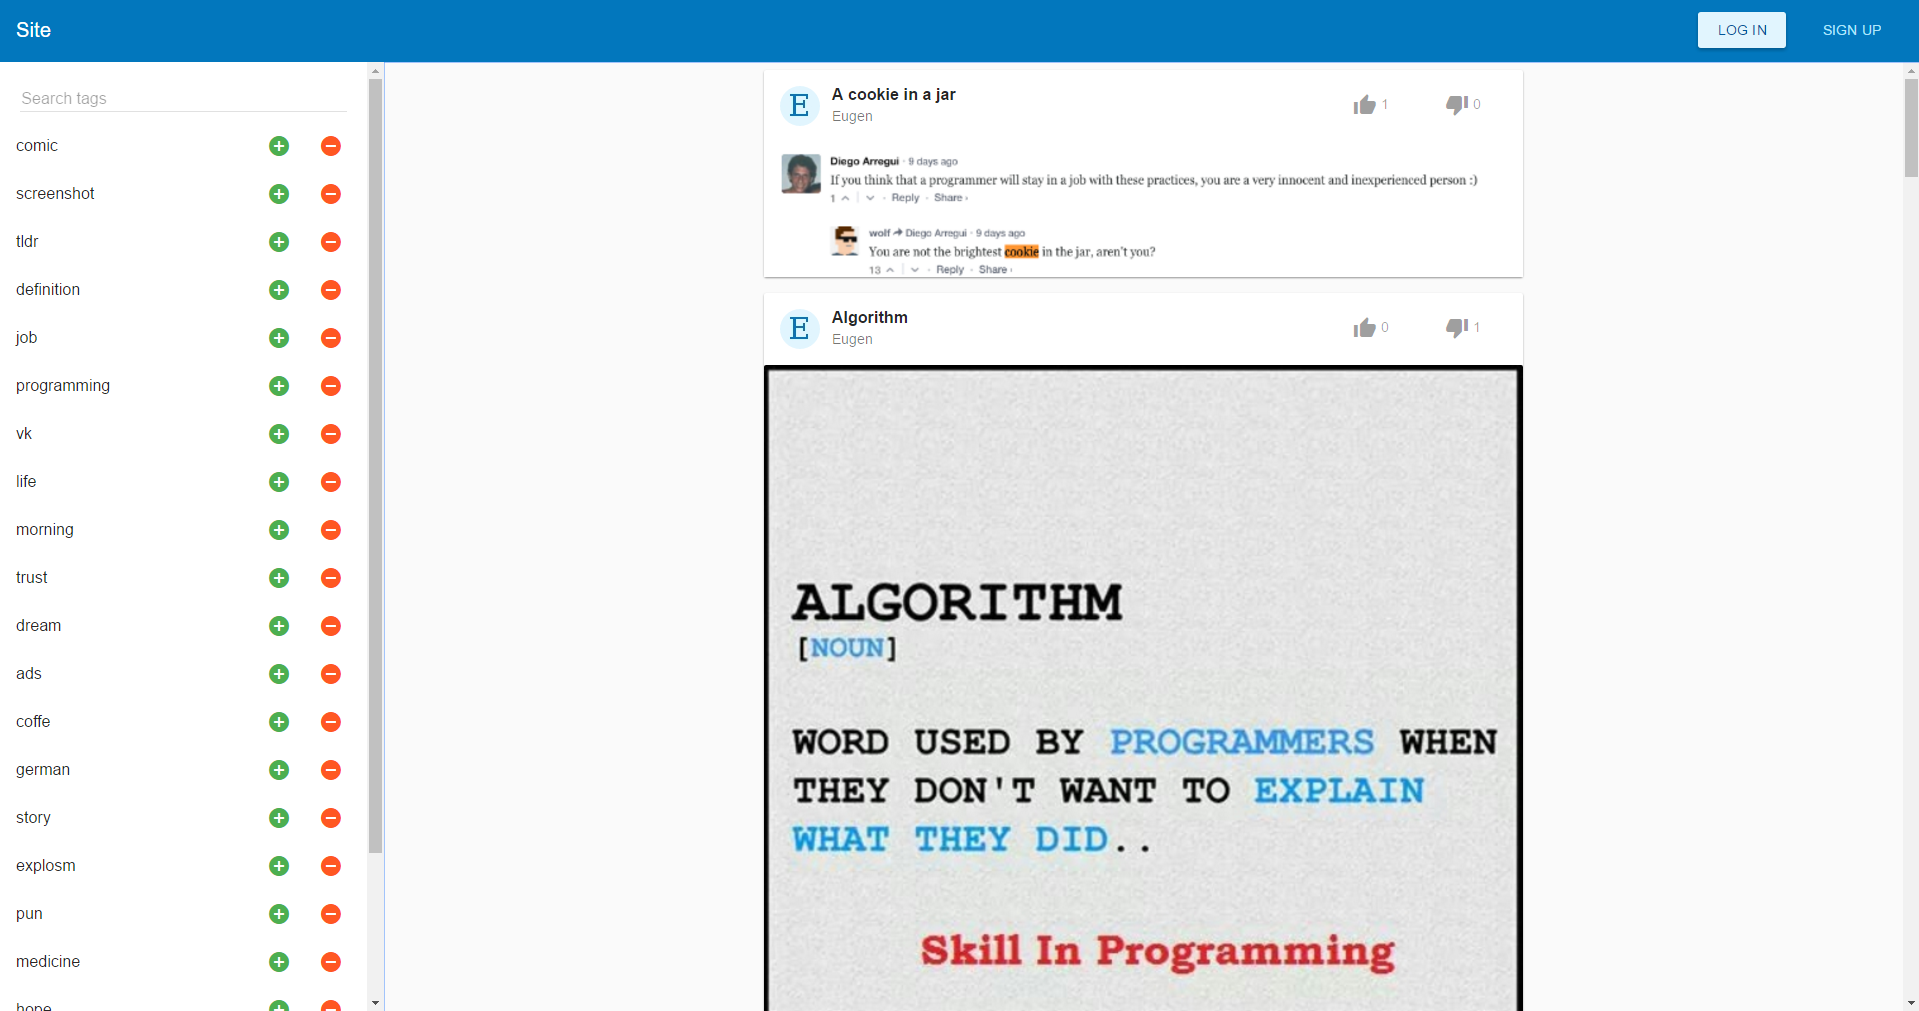
\includegraphics[width=16cm]{home}
	\caption{Pagina principală pe Desktop}
\end{figure}

\begin{figure}[ht]
	\centering
	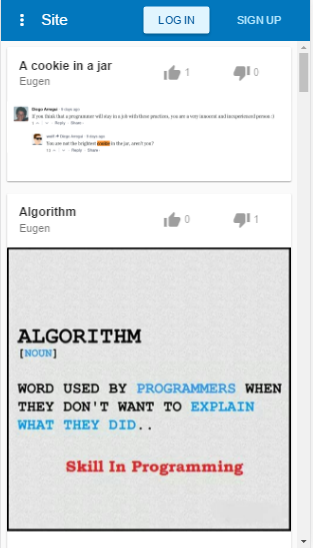
\includegraphics[width=5.5cm]{homeMobile}
	\caption{Pagina principală pe Mobile}
\end{figure}

\begin{figure}[ht]
	\centering
	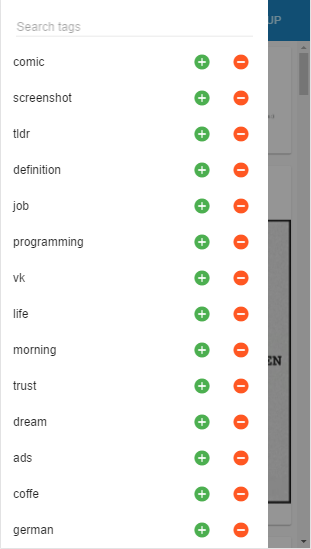
\includegraphics[width=5.5cm]{homeMobileSidebar}
	\caption{Sidebar pe pagina principală de pe dispozitiv Mobile}
\end{figure}

\begin{figure}[ht]
	\centering
	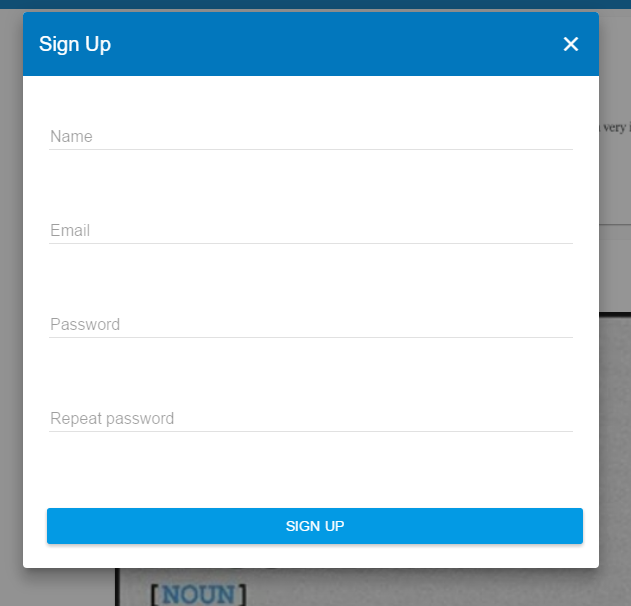
\includegraphics[width=5.5cm]{signup}
	\caption{Pagina de înregistrare}
\end{figure}

\begin{figure}[ht]
	\centering
	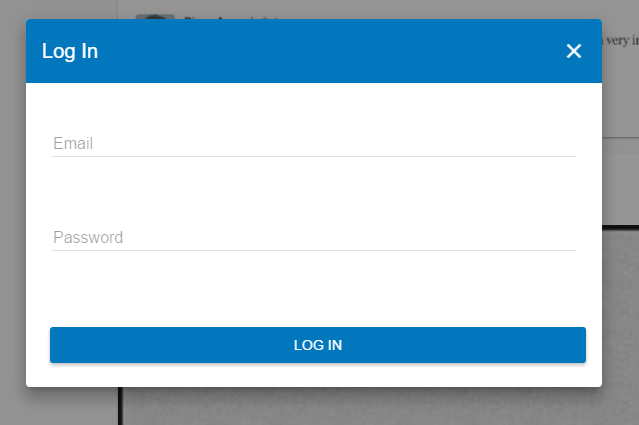
\includegraphics[width=5.5cm]{login}
	\caption{Pagina de autentificare}
\end{figure}

\begin{figure}[ht]
	\centering
	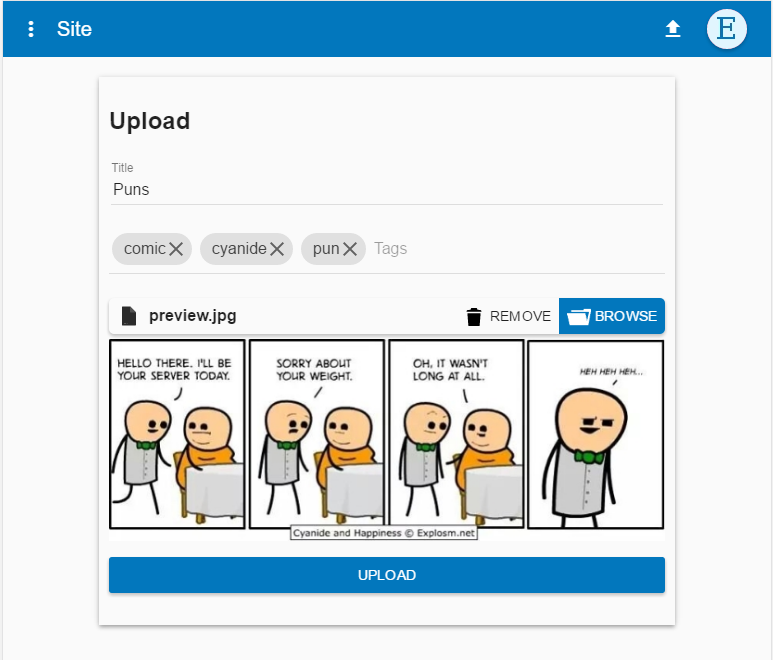
\includegraphics[width=10cm]{upload}
	\caption{Încărcarea unei imagini}
\end{figure}

\begin{figure}[ht]
	\centering
	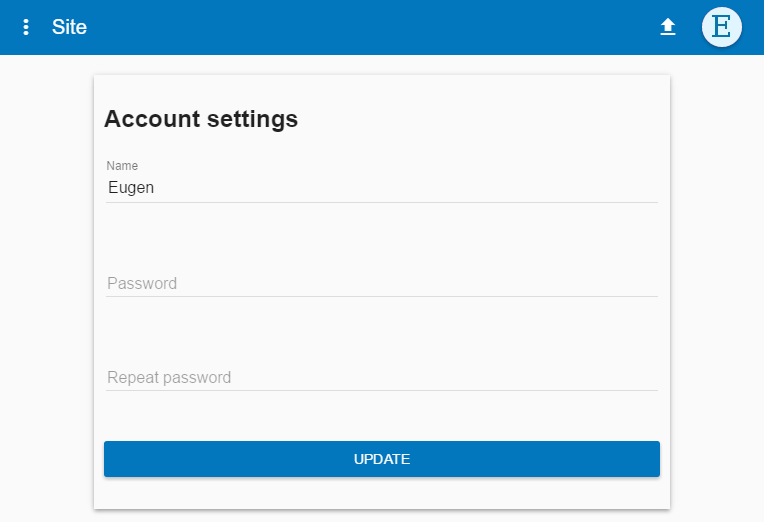
\includegraphics[width=10cm]{account}
	\caption{Modifcarea setărilor de cont}
\end{figure}

\clearpage